\section{Hadoop distributed architecture}

There are a 2 main problems that the hadoop system tries to solve. 
The first is how can we store large amounts of records across multiple machines.
The second is how can we then process those records across multiple machines at once.

Hadoop achieves problem number one by utilizing HDFS (Hadoop distributed file system). 

The second problem is solved by using a technique known as MapReduce.
We will cover HDFS and MapReduce in the following sections. 

So what does a distributed environment look like? At a high level we can see in Figure \ref{fig:distributed} a collection of inter-connected servers. This is the main thing that defines a distributed architecture. 

\begin{figure}[H]
  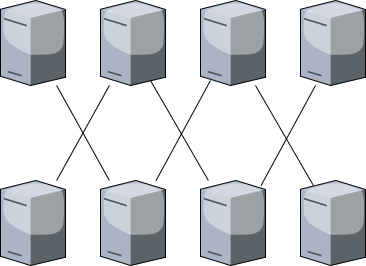
\includegraphics[width=\linewidth]{./images/distributed.png}
  \caption{Distributed Architecture.}
  \label{fig:distributed}
\end{figure}

If we compare this to a single server architecture it becomes clear what the advantages are. In single server we are limited to the RAM/CPU/Storage of one machine. Imagine now we want to scale that machine because we have more users. We would need to buy more ram or newer CPU. This is costly and does not scale well over time. Now we look at the distributed architecture for the same use case of increased users. Instead of having to scale up our RAM/CPU/Storage we can simply add a new server to the cluster. This is less expensive and scales much better. Imagine we have a 4 node cluster. Adding another 4 nodes would effectively double our capacity and processing capability. It is important to note it wont completely double our capacity as there will be some overhead involved in accessing files on x node, but we can say it is very close to 2 times the capacity.
